\section{HybridGuard Design}
\label{sec:system}

\begin{figure*}[t]
  \centering
  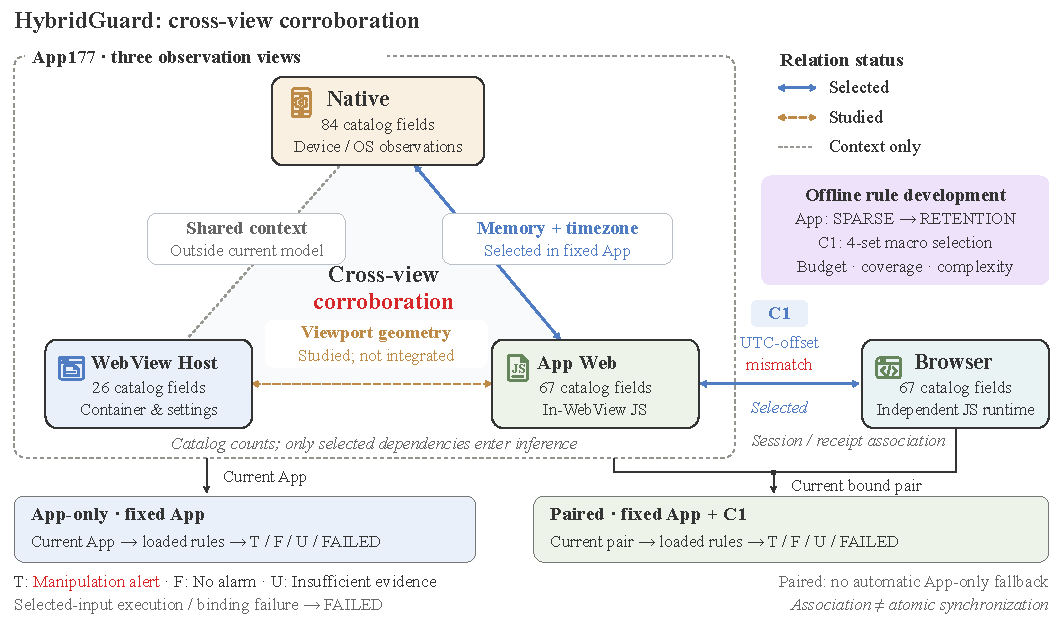
\includegraphics[width=\textwidth]{figures/HybridGuard_overview_triangle.pdf}
  \caption{HybridGuard as a triangle of complementary observation views. Native, WebView Host, and App Web provide device/system, container/settings, and webpage-runtime observations. Solid blue edges denote relations selected in the retained models: Native--App Web memory and timezone relations, and the App Web--independent Browser numeric UTC-offset condition C1. The dashed ochre edge denotes separately studied Host geometry that is not integrated; the arrowless dotted gray edge denotes only shared Native--Host context outside the current App rule pool. Arrowed comparison edges identify the views being compared, not bidirectional rule execution or trusted ground truth. The App detector combines within-view rules with selected cross-view relations. Offline development applies App SPARSE selection and RETENTION, followed by constrained macro-detection selection over four cross-endpoint sets. Separate App-only and paired interfaces load fixed models and read only current inputs. T denotes a manipulation alert, F no alarm, and U insufficient evidence; execution or binding failures in selected inputs take precedence as FAILED. Paired inference has no automatic App-only fallback. Field counts describe catalogs, binding IDs are not detection features, and association does not imply atomic synchronization.}
  \Description{Native, WebView Host, and App Web form a triangle. Selected memory and timezone comparisons use a solid blue edge; separately studied geometry uses a dashed ochre edge. The arrowless dotted gray edge denotes shared context only. The independent Browser is outside the triangle and connected to App Web by C1. Offline development is separate from the two current-input interfaces.}
  \label{fig:hybridguard-overview}
\end{figure*}


Figure~\ref{fig:hybridguard-overview} provides an overview of the observation views and their relationships.

HybridGuard is organized as an auditable chain from collection to relation evidence rather than as a monolithic classifier. The current repository implements the multi-layer collector, backend provenance records, snapshot construction, App evidence extraction, deterministic relation execution, verification, and trace generation. Browser-aware decision logic, a large-scale public benchmark, and calibrated production decisions remain later stages. The architecture nevertheless represents these later stages explicitly so that the current data products can evolve without changing their meaning.

\subsection{Design Principles}

The design begins with a fixed-contract view of fingerprint collection. The active release publishes a versioned field catalog and a corresponding state entry for each signal. Adding, deleting, renaming, or changing the type of a signal requires an explicit schema revision; an older payload is not padded with defaults and relabeled as current. This choice makes the field count meaningful and allows every result to be tied to the exact collector and catalog that produced it.

Fusion is permitted only after provenance has been established. App and external-browser payloads remain independent canonical records in the backend, each with its own receipt and content hash. The system derives a joint view only when the associated batch, receipts, hashes, and pair events close successfully. This ``provenance before fusion'' rule prevents a convenient row-level join from being mistaken for evidence that two observations actually came from the intended collection episode.

Missingness is treated as part of the evidence model rather than as a preprocessing inconvenience. Unsupported APIs, denied permissions, timeouts, runtime errors, and not-applicable relations have different meanings, and the system preserves those meanings through the snapshot and evidence layers. In particular, the absence of an external-browser observation never becomes 67 zero-valued fields. A valid App payload remains usable as App-only evidence, while the missing Browser side is represented in the control plane with an explicit terminal status.

The reasoning path is also deliberately staged. Parsing, normalization, field-family classification, relation applicability, and direct comparisons are computed deterministically before any optional model is involved. Historical LLM prototypes may interpret or summarize this evidence, but they do not define whether an Android version parsed successfully or whether a WebView-provider major version equals a runtime Chromium major version. Finally, labels and shortcut-prone metadata stay outside the runtime. Tool names, provider identities, stable groups, pair roles, splits, and verified facts are used to construct and audit an experiment, not to trigger the relation evaluator.

\subsection{Collection Architecture}

The FeatureApp coordinates the three in-app surfaces. Native code first records Android and device state and captures WebView-host properties. It then loads the versioned Web probe inside the application WebView, receives the JavaScript-visible runtime measurements, and packages the three layers into an \appfp payload together with a collection manifest and per-field states. The backend stores a canonical raw representation, computes or verifies the payload hash, issues a receipt, and associates the record with the current process-lifecycle collection batch. Analysis projections may be generated for convenience, but the canonical raw payload and its receipt remain the authoritative source.

The external-browser path begins only after the App-side collection has enough provenance to request a companion observation. The backend creates a short-lived pairing context, and the application launches the system browser to the independent Web probe. A completed \browserfp upload receives its own raw record and is linked to the initiating App session through pair events and a completed pair-provenance object. The pair record identifies the two canonical payloads; it does not replace them with a new untraceable upload.

The two uploads are asynchronous and may fail independently. This property is important in mobile testing, where browser launch restrictions, foreground transitions, provider behavior, timeouts, and platform support can prevent the companion probe from completing even after a valid App payload has been accepted. HybridGuard therefore produces four logically different products. A provenance-complete App and Browser pair becomes a derived \pairedfp record. A valid App whose Browser attempt is incomplete or unsupported remains in the App-only 177 view. Records that violate release, schema, receipt, batch, hash, or provenance constraints enter quarantine with an explicit reason. Session identifiers, receipts, pair identifiers, batch metadata, and selection decisions are retained in a sample index and audit files rather than mixed into the signal vector.

This separation lets downstream consumers choose an evidence unit honestly. An App-only analysis operates on 177 observed signals and their states. A paired analysis requires the completed 244-field view. Neither path silently changes dimensionality based on convenience, and the failure of one collection surface does not erase valid evidence from another.

\subsection{Evidence and Knowledge Layers}

An accepted App payload is converted into an EvidenceBundle by a deterministic extractor. The bundle does not merely expose the original JSON to a model. It records normalized facts, the source field paths from which those facts were derived, relation prerequisites, status and parsing outcomes, tolerance-relevant context, and a deterministic content hash. Examples include parsed Android and Chromium major versions, platform families, WebView-token presence, default and runtime user-agent structure, graphics-stack families, display geometry, resource buckets, and JavaScript-bridge topology. When a premise cannot be observed or parsed, the bundle carries that limitation forward instead of inventing a comparison result.

HybridGuard then separates knowledge according to both source and execution status. Official-document knowledge records what Android, Chrome, WebView, and Web APIs mean, which values may be reduced or customized, and which security mechanisms exist. Some of these facts support project-derived semantic relations, such as a coarse compatibility requirement between an Android host and a runtime surface or an incompatibility between an Android graphics stack and an explicit Windows/Direct3D WebGL presentation. These relations are not official attack verdicts: they are project inferences that preserve their source cards, premise fields, tolerance, counterexamples, severity, and compilation status.

Empirical device-mined predicates form a separate catalog. They originate from project observations and historical experiments rather than directly from documentation, so their records must identify the data scope that suggested them and the normal counterexamples that constrain them. Historical cases, teacher labels, and model outputs may be retained as optional research material, but they do not define the ground truth for the current controlled experiment. The official-derived and device-mined executable sets are therefore run independently. Their results may overlap, but their alert counts are not summed into a single undifferentiated ``knowledge hit'' score.

\subsection{Verification and Decision Trace}

For every execution, the runtime records the EvidenceBundle version, the available and unavailable fields, the relations considered, the relations skipped as inapplicable, the predicate results, the evidence references supporting each result, and whether any external model was called. A verifier checks that every cited field exists, every cited relation belongs to the frozen catalog, and every asserted relation state is consistent with the executable predicate and its applicability conditions. This step prevents an explanation from claiming a field or rule that was absent from the input.

The resulting DecisionTrace is designed for reproduction and error analysis rather than only for user-facing presentation. It binds the output to the schema, extractor, relation catalogs, optional retrieval context, model and prompt versions when present, and run artifacts. In the current deterministic path, calibrated risk probability remains unset and an external model is not required. The output is therefore best interpreted as structured integrity evidence that can later feed a calibrated policy, not as a production fraud probability.

\subsection{Current Browser Boundary}

The independent Browser path is implemented, but its present role is data governance and audit. The Browser sidecar compares only fields that the frozen policy regards as meaningfully comparable between the in-app Web runtime and the external system browser. Fields whose values are strongly affected by container, process, permission domain, timing, network path, storage state, or browser customization are marked not comparable instead of being forced into a binary same/different decision. Even a recorded difference is an observation, not an attack label.

The active App relation executor does not consume the Browser sidecar, so the current controlled results in Section~\ref{sec:current-results} are strictly \appfp results. Section~\ref{sec:browser-future} describes the normal-pair calibration, release unification, and controlled re-collection required before external-browser evidence can be promoted from an audited data product to an evaluated detection component.
